%!TEX root = /Users/louis/Documents/PhD/Deliverables/Thesis/thesis.tex

\section{MDE Terminology and Principles}
\label{sec:mde_terms}
Software engineers using MDE construct and manipulate artefacts familiar from traditional approaches to software engineering (such as code and documentation) and, in addition, work with different types of artefact, such as \emph{models}, \emph{metamodels} and \emph{model transformations}. Furthermore, model-driven engineering involves new development activities, such as \emph{model management}. This section describes the artefacts and activities typically involved in a model-driven engineering process.

\subsection{Models} % TODO: review Jackson's and Kurtev's definitions of model
When used here, the term \emph{model} has the same meaning as given in \cite{kolovos06eol}: a model is a description of a phenomenon of interest, and may have either a textual or graphical representation. A model provides an abstraction over a real-world object, which enables engineers of differing disciplines to reason about that object.

Abstraction is the primary reason for and the primary goal of modelling. \cite{evans04domain} proposes the use of models throughout the development process to capture and communicate domain knowledge and to shape the structure of the resulting software. Evans emphasises the importance of modelling and a process, which he terms \emph{refactoring to deeper insight}, that seeks incremental improvements to models.

\begin{quote}
Distillation is the process of separating the components of a mixture to extract the essence in a form that makes it more valuable and useful. A model is a distillation of knowledge. With every refactoring to deeper insight, we abstract some crucial aspect of domain knowledge and priorities. \cite[pg397]{evans04domain}
\end{quote}

\cite[ch14]{martin06agile} notes that, in some engineering disciplines, models are used to reduce risk. Structural engineers build models of bridges. Aerospace engineers build models of aircraft. In these disciplines, a model is used to determine the efficacy of the real thing and, moreover, is cheaper to build and test than the real thing, often by a huge factor. The produce of many engineering disciplines is physical and the manufacturing process costly. Often, software models are not cheaper by a huge factor to build and test than the software they represent. Consequently, \cite[ch14]{martin06agile} prescribes software modelling for communicating and reasoning about a design, and not as a long-term replacement for real, working software.

All software has a \emph{domain}, the activities or business of its users. The domain of a library's lending system includes books, people and loans. \cite{evans04domain} prescribes principles and practices for building software in a way that emphasises the underlying domain, while tackling its complexity. In \cite{evans04domain}, domain models are key -- they are used to shape the solution's design, to define a common vocabulary for communication between team members, and to distinguish interesting and uninteresting elements of the domain. According to \cite{evans04domain}, domain models are key to software development. 

% Leading towards this argument:  Model-driven engineering provides principles and practices for defining and using modelling languages. A common metamodelling language is key. Is generative programming?

% How is the situation Martin describes (and other adovcates of "agile" principles) different to the software produced by model-driven engineering? Perhaps for enterprise systems it is much cheaper to build / test a model?? Or perhaps Martin is right, but MDD has different advantages to modelling (e.g. a common metamodelling language).

\subsection{Metamodelling}
In model-driven engineering, models are structured (conform to a well-defined set of syntactic and semantic constraints) rather than unstructured \cite{kolovos09thesis}. A \emph{modelling language} is the set of syntactic and semantic constraints used to define the structure of group of related models. In model-driven engineering, a modelling language is often specified as a model and, hence the term \emph{metamodel} is often used in place of \emph{modelling language}.

Metamodels facilitate model interchange and, hence, interoperability between modelling tools.  For this reason, Evans recommends that software engineers ``use a well-documented shared language that can express the necessary domain information as a common medium of communication.'' \cite[pg377]{evans04domain}. To support this recommendation, Evans discusses Chemical Markup Language (CML), a standardised language, which has facilitated the interoperability of tools (such as JUMBO Browser, which creates graphical views of chemical structures) developed by various institutions.

A metamodel typically comprises three categories of constraint:

\begin{itemize}
	\item \textbf{The concrete syntax} provides a notation for constructing models that conform to the language. For example, a model may be represented as a collection of boxes connected by lines. A standardised concrete syntax enables communication. Concrete syntax may be optimised for consumption by machines (e.g. XML Metadata Interchange (XMI) \cite{xmi}) or by humans (e.g. the concrete syntax of the Unified Modelling Language (UML) \cite{uml212}).
	\item \textbf{The abstract syntax} defines the concepts described by the language, such as classes, packages, datatypes. The representation for these concepts is independent of the concrete syntax. For example, compilers may elect to use an abstract syntax tree to encode the abstract syntax of a program (whereas the concrete syntax for the same language may be textual or diagrammatic).
	\item \textbf{The semantics} identifies the meaning of the modelling concepts in the particular domain of language. For example, consider a modelling language defined to describe genealogy, and another to describe flora. Although both languages may define a tree construct, the semantics of a tree in one is likely to be different from the semantics of a tree in the other. The semantics of a modelling language may be specified rigorously, by defining a reference semantics in a formal language such as Z \cite{z}, or in a semi-formal manner by employing natural language.
\end{itemize}

Concrete syntax, abstract syntax and semantics are used together to specify modelling languages. There are many other ways of defining languages, but this approach (first formalised in \cite{alvarez01mml}) is common in model-driven engineering: a metamodel is often used to define abstract syntax, a grammar or text-to-model transformation to specify concrete syntax, and code generators, annotated grammars or behavioural models to effect semantics.

\subsubsection{MOF}
Software engineers using model-driven engineering can use existing and define new metamodels. To facilitate interoperability between model-driven engineering tools, the OMG has standardised a language for specifying metamodels, the meta-object facility (MOF). Metamodels specified in MOF can be interchanged between model-driven engineering environments. Furthermore, modelling language tools are interoperable because MOF also standardises the way in which metamodels and their models are persisted to and from disk. For model and metamodel persistence MOF prescribes XML Metadata Interchange (XMI), a dialect of XML optimised and standardised by the OMG for loading, storing and exchanging models.

Because MOF is a modelling language for describing modelling languages, it is sometimes termed a metamodelling language. A simplified fragment of the UML defined in MOF, is shown in Figure \ref{fig:mof}. The concrete syntax of MOF borrows is similar to the concrete syntax of UML class diagrams:

\begin{itemize}
 \item Modelling constructs are drawn as boxes. The name of each modelling construct is emboldened. The name of abstract (uninstantiable) constructs are italicised.
 \item Attributes are contained within the box of their modelling construct. Each attribute has a name, a type (prefixed with a colon) and may define a default value (prefixed with an equals sign).
 \item Generalisation is represented using a line with an open arrow-head.
 \item References are specified using a line. An arrow illustrates the direction in which the reference may be traversed (no arrow indicates bi-directionality). Labels are used to name and define the multiplicity of references.
 \item Containment references are specified by including a solid diamond on the containing end.
\end{itemize}

\begin{figure}[htbp]
  \begin{center}
    \leavevmode
    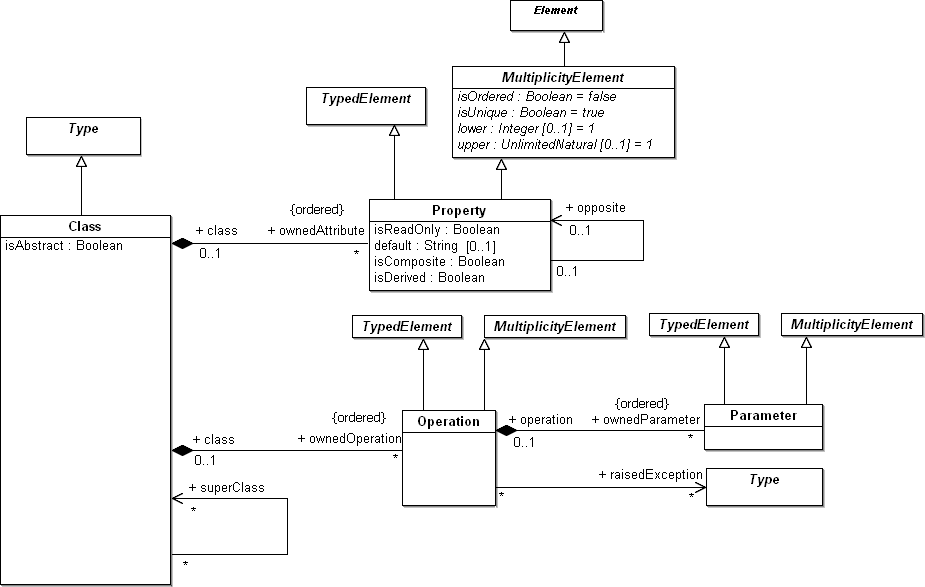
\includegraphics[scale=0.33]{mof.png}
  \end{center}
  \caption{A fragment of the UML metamodel defined in MOF, from \cite{uml212}.}
  \label{fig:mof}
\end{figure}

In the past, the means for describing modelling constructs has been inconsistent between modelling languages. For example, both entity-relationship (ER) diagrams and UML class diagrams can be used to specify models of structured data but, as \cite[pg97]{frankel02mda} notes, similar constructs from ER diagrams and UML class diagrams have different concrete syntax. MOF seeks to standardise the way in which modelling languages are defined.


\subsection{Model-Driven Engineering}
\label{sec:mde}
Model-driven engineering (MDE) is a principled approach to software engineering in which models are produced throughout the engineering process. Models are manipulated throughout development to produce software. This thesis uses the term \emph{model management}, defined in \cite{kolovos09thesis}, to refer to development activities that manipulate models for the purpose of producing software. Typical model management activities are discussed in this section.

\subsubsection{Model Transformation}

\paragraph{Model-to-Model Transformation}

\paragraph{Model-to-Text Transformation}

\paragraph{Text-to-Model Transformation}

\subsubsection{Model Validation}

\subsubsection{Model Comparison}

\subsubsection{Model Merging}


